\documentclass[12pt]{scrartcl}
\usepackage{graphicx}
\usepackage{amsmath}

\begin{document}

%Title section

\titlehead{CS department, Technion}
\subject{Introduction to Optimization and Deep Learning 236330}
\title{HW 3}
\subtitle{Quasi-Newton BFGS method and DNN training}
\author{Uri Kirstein 311137095 \hfill sukirstn@campus.technion.ac.il\and Pavel Rastopchin 321082026 pavelr@campus.technion.ac.il}
\date{\today}
\maketitle

 %end of title section
\section*{Part 1 - BFGS}
\subsection*{Task 2}
We chose $N=10$. Our starting point was $x_0=(0,0,..0)$. We know that a local minimum of the function exists at $x^*=(1,1,...)$ and that $p^*=0$ (our function is non-negative so this must be a global minimum as well). We stopped after 97 iterations at\\\\
$x_{final}$=[ 5.51033772e-07,  6.67959021e-07, -4.45033926e-06, 
2.72106755e-06, 1.86952265e-06, -7.31025632e-09, -1.21113396e-06, -5.86666139e-06, 4.51107833e-06, -5.76553427e-07]\\\\
The error function and gradient at this point are $$f(x_{final})-p^*=5.359357003868173e-14$$
$\nabla f(x_{final})=$[ 5.51033772e-07  6.67959021e-07 -4.45033926e-06  2.72106755e-06\\
  1.86952265e-06 -7.31025632e-09 -1.21113396e-06 -5.86666139e-06
  4.51107833e-06\\ -5.76553427e-07]
$$||\nabla f(x_{final})|| = 9.381977770909129e-06$$
We can see in the graph below that the error function $f(x_k)-p^*$, where $k$ is the number of iterations, is monotonously decreasing. This means we always advance in the direction of the minimum.
\begin{figure}[ht!]
	\hfill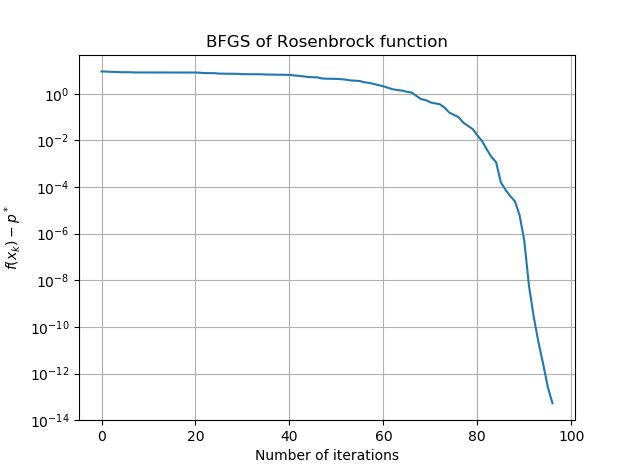
\includegraphics[width=\linewidth]{rosenbrock_graph.jpg}\hspace*{\fill}
	\caption{Task 2}
\end{figure}

\section*{Part 2 - Deep Neural Network}
\subsection*{Task 3}
\begin{align*}
\Psi(r_i)&=r_i^2\\
&=[F(x^i,w)-y_i]^2\\
&=w_3^T\phi_2[w_2^T\phi_1(w_1^Tx^i+b_1)+b_2]+b_3 -x_1^i exp[-(x_1^i)^2-(x_2^i)^2]
\end{align*}
$$\nabla_{w_1}\Psi=\frac{\partial}{\partial w_1}[w_3^T\phi_2w_2^T\phi_1w_1^Tx^i]$$
Notice that $w_3^T\phi_2$, $w_2^T\phi_1$ and $w_1^Tx^i$ are all scalar. As such:
$$w_3^T\phi_2w_2^T\phi_1w_1^Tx^i = Trace(w_3^T\phi_2w_2^T\phi_1w_1^Tx^i)$$
And because of the cyclic property of the trace:
$$Trace(w_3^T\phi_2w_2^T\phi_1w_1^Tx^i)=Trace(w_1^Tx^iw_3^T\phi_2w_2^T\phi_1)=w_1^Tx^iw_3^T\phi_2w_2^T\phi_1$$
We are going to use this trick in many of the partial derivatives. Resuming our calculation:
$$\nabla_{w_1}\Psi=\frac{\partial}{\partial w_1}[w_1^Tx^iw_3^T\phi_2w_2^T\phi_1]$$

Remembering that $x^Ty=y^Tx$ as they are an inner product we get:
$$\nabla_{w_1}\Psi=\frac{\partial}{\partial w_1}[\phi_1^Tw_2\phi_2^Tw_3{x^i}^Tw_1]=\phi_1^Tw_2\phi_2^Tw_3{x^i}^T$$

Remembering that $w_3^T\phi_2$ and $w_2^T\phi_1$ are scalars we can write:
$$\nabla_{w_1}\Psi=w_2^T\phi_1w_3^T\phi_2{x^i}^T$$

\begin{center}
\boxed{\nabla_{w_1}\Psi=w_2^T\phi_1w_3^T\phi_2{x^i}^T}
\end{center}

Using similar methods, we can find the rest of the derivatives.
\begin{align*}
\nabla_{w_2}\Psi&=\frac{\partial}{\partial w_2}[w_3^T\phi_2w_2^T\phi_1(w_1^Tx^i+b_1)]=\frac{\partial}{\partial w_2}[w_2^T\phi_1(w_1^Tx^i+b_1)w_3^T\phi_2]\\
&=\frac{\partial}{\partial w_2}[\phi_1(w_1^Tx^i+b_1)w_3^T\phi_2\phi_1^Tw_2]
\end{align*}

\begin{center}
\boxed{\Rightarrow \nabla_{w_2}\Psi = \phi_1(w_1^Tx^i+b_1)w_3^T\phi_2\phi_1^T}
\end{center}

$$\nabla_{w_3}\Psi=\frac{\partial}{\partial w_2}[w_3^T\phi_2(w_2^T\phi_1(w_1^Tx^i+b_1)+b_2)]=\frac{\partial}{\partial w_2}[(w_2^T\phi_1(w_1^Tx^i+b_1)+b_2)\phi_2^Tw_3]$$

\begin{center}
\boxed{\Rightarrow \nabla_{w_3}\Psi = (w_2^T\phi_1(w_1^Tx^i+b_1)+b_2)\phi_2^T}
\end{center}

\begin{center}
\boxed{\nabla_{b_1}\Psi = w_3^T\phi_2w_2^T\phi_1}
\end{center}

\begin{center}
\boxed{\nabla_{b_2}\Psi = w_3^T\phi_2}
\end{center}

\begin{center}
\boxed{\nabla_{b_3}\Psi = 1}
\end{center}

\end{document}
